\documentclass[tikz,border=12pt]{standalone}
\usepackage[T1]{fontenc}
\usepackage{mathpazo}
\usepackage{amsmath,amssymb}
\usetikzlibrary{arrows.meta, positioning, calc}

\definecolor{stblue}{HTML}{7B97AD}
\definecolor{rwgold}{HTML}{B8995E}
\definecolor{sage}{HTML}{7A9A7E}
\definecolor{dkbrown}{HTML}{3D3530}
\definecolor{wmgray}{HTML}{7B7067}
\definecolor{cream}{HTML}{F9F6F0}
\definecolor{border}{HTML}{D4C9B8}
\definecolor{terracotta}{HTML}{C47A6A}

\begin{document}
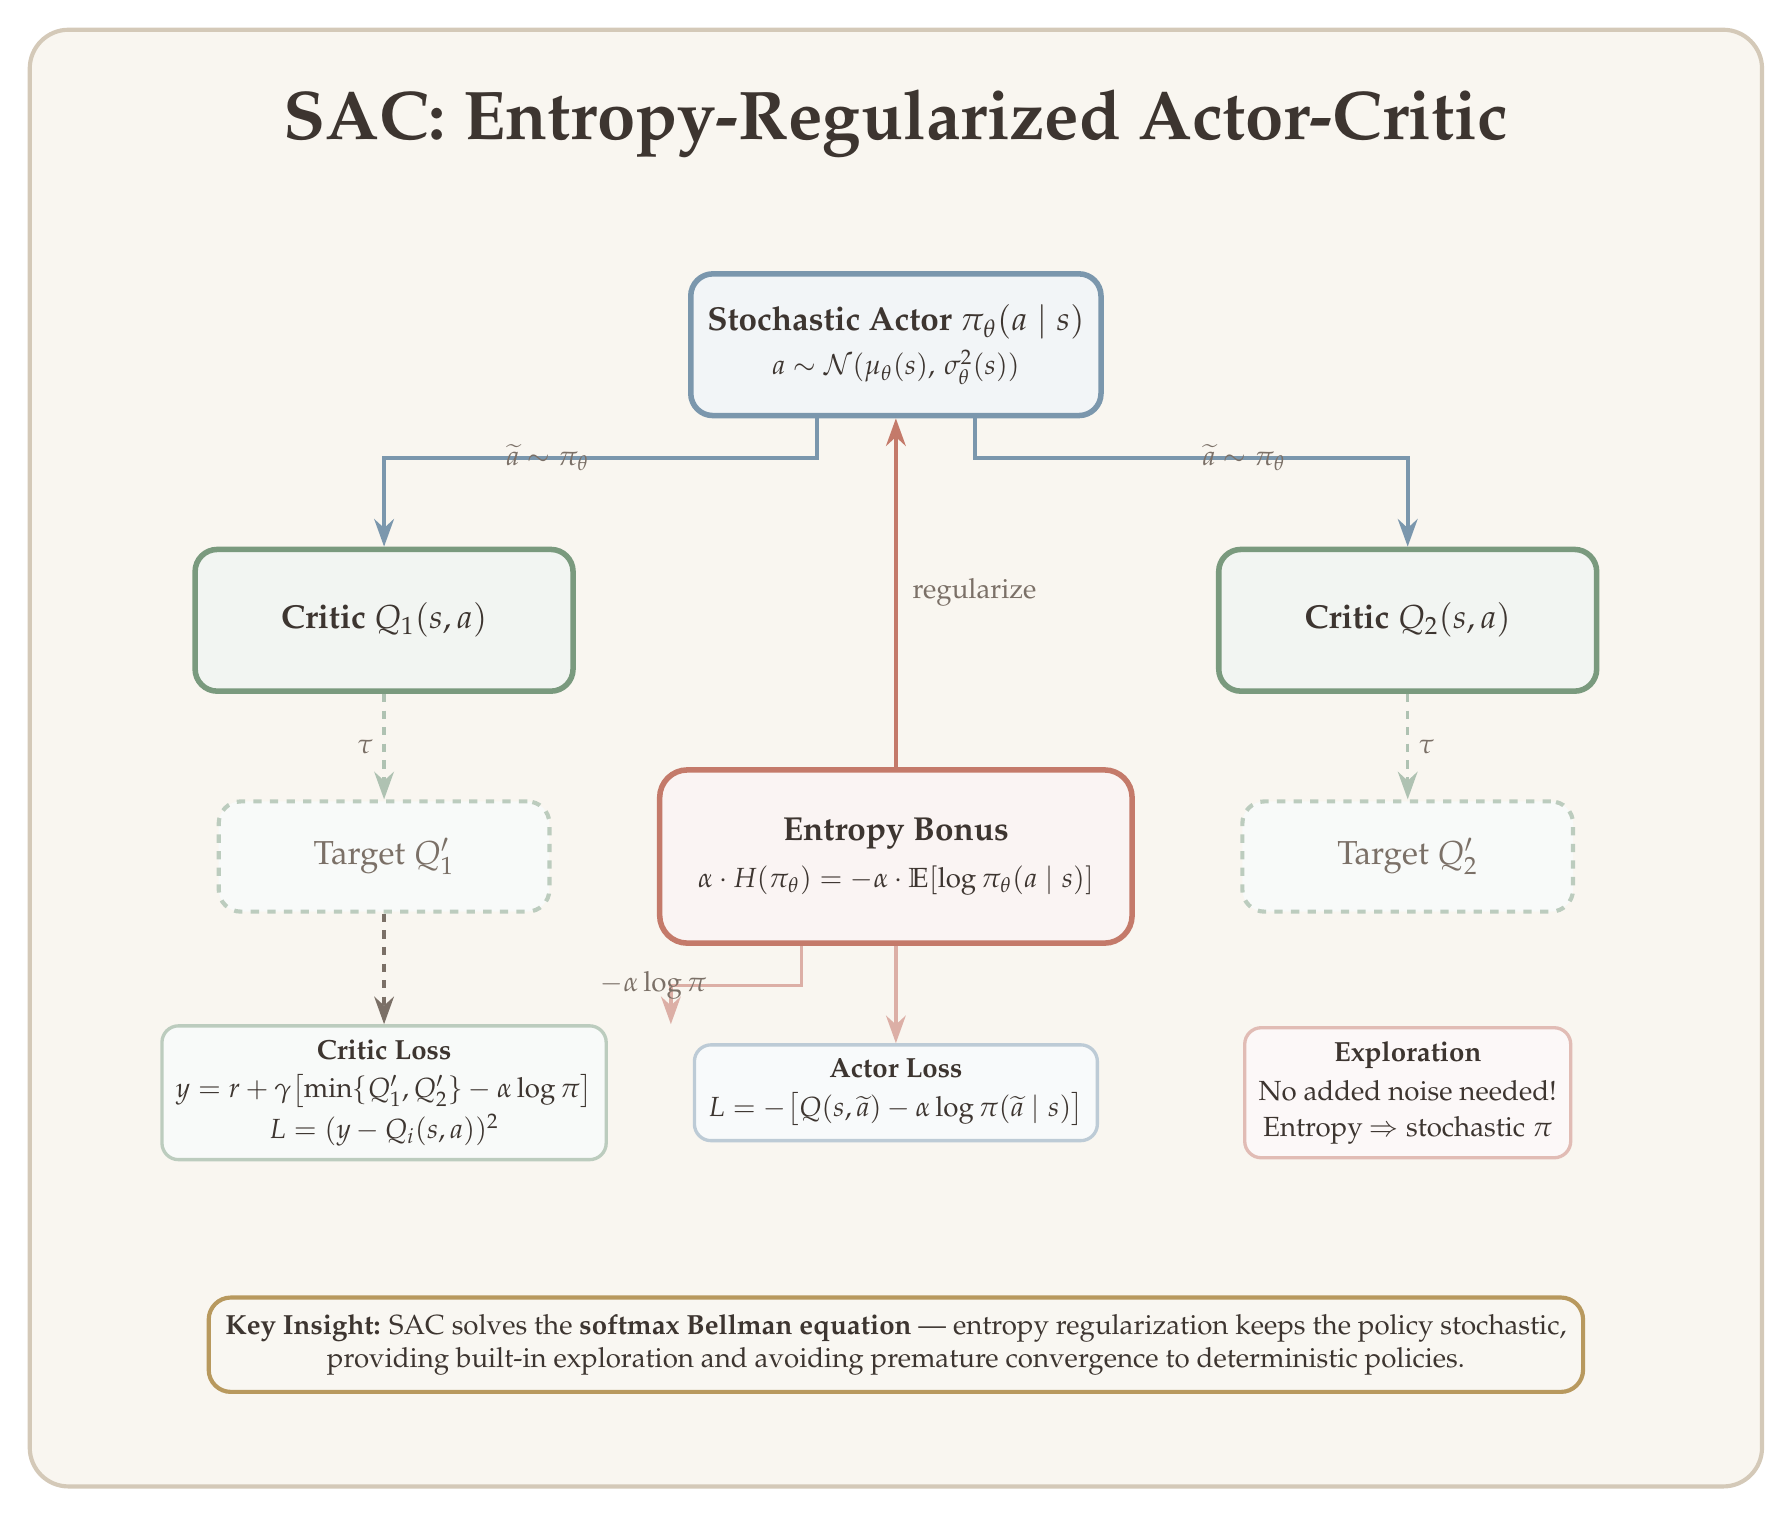
\begin{tikzpicture}[
  >={Stealth[length=3.5mm, width=2.5mm]},
  netbox/.style={
    draw=#1, line width=2pt, fill=#1!10, rounded corners=8pt,
    minimum width=48mm, minimum height=18mm, font=\large, text=dkbrown,
    align=center, inner sep=6pt
  },
  lbl/.style={font=\normalsize, text=wmgray, align=center},
]

% Background
\fill[cream, rounded corners=14pt] (-1,-10) rectangle (21,8.5);
\draw[border, rounded corners=14pt, line width=1.5pt] (-1,-10) rectangle (21,8.5);

% Title
\node[font=\Huge\bfseries, text=dkbrown] at (10,7.3)
  {SAC: Entropy-Regularized Actor-Critic};

% =============================================
% Stochastic Actor (center top)
% =============================================
\node[netbox=stblue] (actor) at (10,4.5)
  {\textbf{Stochastic Actor} $\pi_\theta(a \mid s)$\\[2pt]
   {\normalsize $a \sim \mathcal{N}(\mu_\theta(s),\, \sigma_\theta^2(s))$}};

% =============================================
% Twin Critics
% =============================================
\node[netbox=sage] (q1) at (3.5,1)
  {\textbf{Critic} $Q_1(s, a)$};
\node[netbox=sage] (q2) at (16.5,1)
  {\textbf{Critic} $Q_2(s, a)$};

% =============================================
% Target Critics (dashed)
% =============================================
\node[draw=sage!50, line width=1.5pt, fill=sage!5, rounded corners=8pt,
      minimum width=42mm, minimum height=14mm, font=\large, text=wmgray,
      align=center, inner sep=5pt, dashed]
  (q1t) at (3.5,-2)
  {Target $Q_1'$};
\node[draw=sage!50, line width=1.5pt, fill=sage!5, rounded corners=8pt,
      minimum width=42mm, minimum height=14mm, font=\large, text=wmgray,
      align=center, inner sep=5pt, dashed]
  (q2t) at (16.5,-2)
  {Target $Q_2'$};

% =============================================
% Entropy bonus
% =============================================
\node[draw=terracotta, line width=2pt, fill=terracotta!8, rounded corners=10pt,
      minimum width=60mm, minimum height=22mm, font=\large, text=dkbrown,
      align=center, inner sep=6pt]
  (entropy) at (10,-2)
  {\textbf{Entropy Bonus}\\[3pt]
   {\normalsize $\alpha \cdot H(\pi_\theta) = -\alpha \cdot \mathbb{E}[\log \pi_\theta(a \mid s)]$}};

% =============================================
% Loss equations
% =============================================
\node[draw=sage!50, line width=1.2pt, fill=sage!5, rounded corners=6pt,
      font=\normalsize, text=dkbrown, align=center, inner sep=5pt]
  (closs) at (3.5,-5)
  {\textbf{Critic Loss}\\[2pt]
   $y = r + \gamma\bigl[\min\{Q_1', Q_2'\} - \alpha\log\pi\bigr]$\\[1pt]
   $L = (y - Q_i(s,a))^2$};

\node[draw=stblue!50, line width=1.2pt, fill=stblue!5, rounded corners=6pt,
      font=\normalsize, text=dkbrown, align=center, inner sep=5pt]
  (aloss) at (10,-5)
  {\textbf{Actor Loss}\\[2pt]
   $L = -\bigl[Q(s, \widetilde{a}) - \alpha\log\pi(\widetilde{a} \mid s)\bigr]$};

\node[draw=terracotta!50, line width=1.2pt, fill=terracotta!5, rounded corners=6pt,
      font=\normalsize, text=dkbrown, align=center, inner sep=5pt]
  (explore) at (16.5,-5)
  {\textbf{Exploration}\\[2pt]
   No added noise needed!\\[1pt]
   Entropy $\Rightarrow$ stochastic $\pi$};

% =============================================
% Key insight box
% =============================================
\node[draw=rwgold, line width=1.5pt, fill=rwgold!8, rounded corners=8pt,
      font=\normalsize, text=dkbrown, align=center, inner sep=6pt]
  (key) at (10,-8.2)
  {\textbf{Key Insight:} SAC solves the \textbf{softmax Bellman equation} ---
   entropy regularization keeps the policy stochastic,\\
   providing built-in exploration and avoiding premature convergence to deterministic policies.};

% =============================================
% Arrows
% =============================================

% Actor -> Critics (provides actions)
\draw[->, line width=1.5pt, stblue] ([xshift=-10mm]actor.south) -- ++(0,-0.5) -| (q1.north)
  node[pos=0.25, left, lbl] {$\widetilde{a} \sim \pi_\theta$};
\draw[->, line width=1.5pt, stblue] ([xshift=10mm]actor.south) -- ++(0,-0.5) -| (q2.north)
  node[pos=0.25, right, lbl] {$\widetilde{a} \sim \pi_\theta$};

% Critics -> target critics (soft update)
\draw[->, line width=1.2pt, dashed, sage!60] (q1.south) -- (q1t.north)
  node[midway, left, lbl] {$\tau$};
\draw[->, line width=1.2pt, dashed, sage!60] (q2.south) -- (q2t.north)
  node[midway, right, lbl] {$\tau$};

% Entropy -> Actor (regularizes)
\draw[->, line width=1.5pt, terracotta] (entropy.north) -- (actor.south)
  node[midway, right, lbl, xshift=2pt] {regularize};

% Target critics -> critic loss
\draw[->, line width=1.2pt, dashed, wmgray] (q1t.south) -- (closs.north);

% Entropy -> critic loss (entropy in target)
\draw[->, line width=1.2pt, terracotta!60] ([xshift=-12mm]entropy.south) -- ++(0,-0.5) -| ([xshift=8mm]closs.north east)
  node[pos=0.3, left, lbl, xshift=-2pt] {$-\alpha\log\pi$};

% Entropy -> actor loss
\draw[->, line width=1.2pt, terracotta!60] (entropy.south) -- (aloss.north);

\end{tikzpicture}
\end{document}
